\newcommand{\decal}[5]{
\begin{minipage}{\linewidth}
	\begin{minipage}[t]{0.3\textwidth}
       \vspace{0pt}
	\ifthenelse{\isodd{#1}}{
		\includegraphics[width=0.9\textwidth,page=#1,viewport=103 #3 291 #4,clip=true]{13GR_PistopioimeniSimansi_ISO_7010.pdf}
	}{
		\includegraphics[width=0.9\textwidth,page=#1,viewport=70 #3 261 #4,clip=true]{13GR_PistopioimeniSimansi_ISO_7010.pdf}
	}
	\end{minipage}
	\begin{minipage}[t]{0.6\textwidth}
\setlength{\parindent}{4em}
\setlength{\parskip}{1.2em}
       \vspace{0pt}\raggedright
	{\LARGE \textbf{#2}}
	
	
	#5
	\vspace{1cm}
	\end{minipage}
\end{minipage}
}
\newcommand{\action}[3]{\decal{#1}{#2}{520}{715}{#3}}
\newcommand{\prohib}[3]{\decal{#1}{#2}{495}{690}{#3}}
\newcommand{\warn}[3]{\decal{#1}{#2}{520}{715}{#3}}

\newcommand{\machinePage}[6]{%
\begin{center}
\vspace{0cm}
{\fontsize{50}{60} \textbf{#1}}
 
\action{49}{\textbf{%
 	\IfSubStr{#2}{Approval}%
		{Instructions \& Approval Mandatory}
		{Instructions Mandatory}%
}}{%
Instructions \textbf{prior} to use are mandatory. Check the wiki for whom can help you.

#3


\IfSubStr{#2}{Noise}{Machine can only be used between 07:00 - 19:00 (be kind to our neighbours).}


\IfSubStr{#2}{Approval}{Must have the `dangerous equipment waiver' filed with the foundations trustees and been given approval or card access.}{}

\IfSubStr{#2}{Two}{A second person must be present during operation. This person must have agreed to be your second and needs to know how to stop the machine.}

}
\begin{minipage}{\linewidth}
	\begin{minipage}[t]{0.5\textwidth}\vspace{0pt}#4\end{minipage}
	\begin{minipage}[t]{0.5\textwidth}\vspace{0pt}#5\end{minipage}
\end{minipage}
\vspace{0.2cm}

#6

If the machine is not clean or appears broken - then report this to the mailing list. Clean/fix prior to use.

\textbf{Report any damage, issues or accident within 24 hours to the mailing list.}
\end{center}
\pagebreak
}

